This section provides a complete analysis of the NSL-KDD dataset.

%-------
\subsection{Dataset Summary}

The NSL-KDD dataset is provided in two forms: \texttt{.arff} files, with binary labels, and \texttt{.csv} files, with categorical labels for each instance.

Since the object of this work is to build a binary classifier, we will focus only on the \texttt{.arff} files. The provided \texttt{.arff} files are:

\begin{itemize}
    \item \textbf{KDDTrain+.ARFF}: The full NSL-KDD train set with binary labels in ARFF format
    \item \textbf{KDDTrain+\_20Percent.ARFF}: A 20\% subset of the KDDTrain+.arff file
    \item \textbf{KDDTest+.ARFF}: The full NSL-KDD test set with binary labels in ARFF format
    \item \textbf{KDDTest-21.ARFF}: A subset of the KDDTest+.arff file which does not include records with difficulty level of 21 out of 21
\end{itemize}

To avoid redundancy, we use only the \texttt{KDDTrain+.ARFF} and \texttt{KDDTest+.ARFF} files, which contain a total of about 148,500 entries.

Table~\ref{tab:summ} contains a summary of the most important attributes of the dataset.

\FloatBarrier

\begin{table}[!htb]
    \centering
    
    \begin{tabular}{|l|l|}
    \hline
    \multicolumn{2}{|c|}{\textbf{Summary}} \\ \hline
    train rows              & 125973             \\ \hline
    test rows               & 22544              \\ \hline
    total rows              & 148517             \\ \hline
    columns                 & 42                 \\ \hline
    duplicates              & 629                \\ \hline
    null values             & None               \\ \hline
    \end{tabular}
    \caption{Dataset Attributes}
    \label{tab:summ}
\end{table}
\FloatBarrier

%-------
\subsection{Features}
            
As for the features of this dataset, they can be broken down into 4 types (excluding the target column):

\begin{itemize}
    \item 4 Multi-Class
    \item 6 Binary
    \item 16 Discrete
    \item 15 Continuous
\end{itemize}

Tables~\ref{tab:cat} and \ref{tab:bin} contain a description of the categorical features of the dataset, while Tables~\ref{tab:disc} and \ref{tab:cont} describe the numerical features. Note that this definition slightly differs from the one provided by \cite{nslkdd}, since here categorical and binary features are listed regardless of their format (text or numeric). 
\begin{table}[]
    \centering
    \begin{tabular}{|l|l|}
    \hline
    \multicolumn{2}{|c|}{\textbf{Multi-Class Features}} \\ \hline
    \textit{Feature}     & \textit{Distinct Values} \\ \hline
    protocol\_type        & 3                \\ \hline
    service               & 70               \\ \hline
    flag                  & 11               \\ \hline
    su\_attempted	      & 3                \\ \hline
    \end{tabular}
    \caption{Multi-Class Features in the NSL-KDD dataset}
    \label{tab:cat}
\end{table}

\begin{table}[]
    \centering
    \begin{tabular}{|l|l|}
    \hline
    \multicolumn{2}{|c|}{\textbf{Binary Features}} \\ \hline
    \textit{Feature}     & \textit{Number of '0's} \\ \hline
    land	 & 99.98\%	 \\ \hline
    logged\_in	 & 59.72\%	 \\ \hline
    root\_shell	 & 99.85\%	 \\ \hline
    num\_outbound\_cmds	 & 100.00\%	 \\ \hline
    is\_host\_login	 & 99.99\%	 \\ \hline
    is\_guest\_login	 & 98.77\%	 \\ \hline
    \end{tabular}
    \caption{Binary Features in the NSL-KDD dataset}
    \label{tab:bin}
\end{table}

\begin{table}[]
    \centering
     \begin{tabular}{|l|l|l|}
    \hline
    \multicolumn{3}{|c|}{\textbf{Discrete Features}} \\ \hline
    \textit{Feature}     & \textit{Mean} & \textit{Stddev} \\ \hline
    wrong\_fragment   & 0.02      & 0.24  \\ \hline
    urgent   & 0.00      & 0.02  \\ \hline
    count    & 83.34     & 116.76    \\ \hline
    srv\_count    & 28.25     & 75.37     \\ \hline
    dst\_host\_count   & 183.93    & 98.53     \\ \hline
    dst\_host\_srv\_count   & 119.46    & 111.23    \\ \hline
    duration     & 276.78    & 2.46k   \\ \hline
    src\_bytes    & 40.22k      & 5.4M    \\ \hline
    dst\_bytes    & 17.08k     & 3.7M    \\ \hline
    hot  & 0.19      & 2.01  \\ \hline
    num\_failed\_logins    & 0.00      & 0.07  \\ \hline
    num\_compromised  & 0.26      & 22.23     \\ \hline
    num\_root     & 0.27      & 22.69     \\ \hline
    num\_file\_creations   & 0.01      & 0.52  \\ \hline
    num\_shells   & 0.00      & 0.03  \\ \hline
    num\_access\_files     & 0.00      & 0.10  \\ \hline
    \end{tabular}
    \caption{Discrete Features in the NSL-KDD dataset}
    \label{tab:disc}
\end{table}

\begin{table}[]
    \centering
    \begin{tabular}{|l|l|l|}
    \hline
    \multicolumn{3}{|c|}{\textbf{Continuous Features}} \\ \hline
    \textit{Feature}     & \textit{Mean} & \textit{Stddev} \\ \hline
    serror\_rate  & 0.26      & 0.43  \\ \hline
    srv\_serror\_rate  & 0.26      & 0.43  \\ \hline
    rerror\_rate  & 0.14      & 0.34  \\ \hline
    srv\_rerror\_rate  & 0.14      & 0.34  \\ \hline
    same\_srv\_rate    & 0.67      & 0.44  \\ \hline
    diff\_srv\_rate    & 0.07      & 0.19  \\ \hline
    srv\_diff\_host\_rate   & 0.10      & 0.26  \\ \hline
    dst\_host\_same\_srv\_rate   & 0.53      & 0.45  \\ \hline
    dst\_host\_diff\_srv\_rate   & 0.08      & 0.19  \\ \hline
    dst\_host\_same\_src\_port\_rate  & 0.15      & 0.31  \\ \hline
    dst\_host\_srv\_diff\_host\_rate  & 0.03      & 0.11  \\ \hline
    dst\_host\_serror\_rate     & 0.26      & 0.43  \\ \hline
    dst\_host\_srv\_serror\_rate     & 0.25      & 0.43  \\ \hline
    dst\_host\_rerror\_rate     & 0.14      & 0.32  \\ \hline
    dst\_host\_srv\_rerror\_rate     & 0.14      & 0.34  \\ \hline
    \end{tabular}
    \caption{Continuous Features in the NSL-KDD dataset}
    \label{tab:cont}
\end{table}



%-------
\subsection{Categories Distributions}

The NSL-KDD dataset contains a few binary and multi-class categorical features, which are used to label each connection with its protocol, service and other useful characteristics, e.g. if the user tried to gain super-user access or if he spawned a root shell during its connection. 

The figures contained in the next page describe, for each categorical feature, how many occurrences of each label are present in both the train and the test set. Note that \textit{class}, \textit{protocol\_type}, \textit{service} and \textit{flag} features contain textual values, while all other categories are expressed by a number.

As we can see, the target variable (\textit{class}) has a nearly even distribution of its values (\textit{normal} and \textit{anomalous)} throughout the dataset, meaning that there are a lot of anomalous examples that can be used for training. As opposed to this, we can see that some of the categories are not evenly distributed, having more than 99\% of the samples belonging to just one class. This kind of analysis can be useful during the feature selection step.


\FloatBarrier

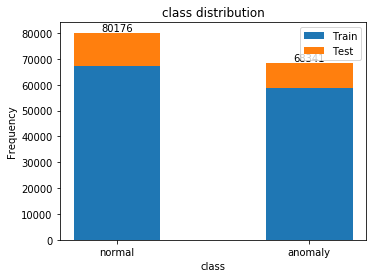
\includegraphics[width=0.9\linewidth]{img/cat6.png}


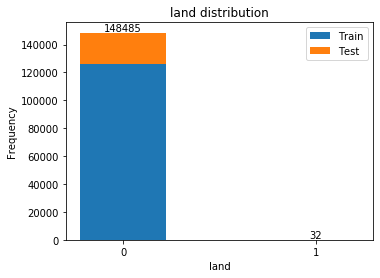
\includegraphics[width=0.9\linewidth]{img/cat1.png}

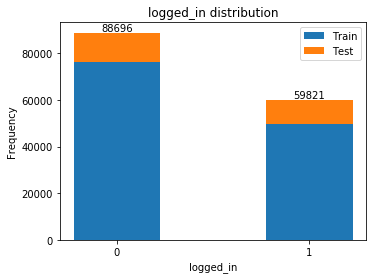
\includegraphics[width=0.9\linewidth]{img/cat2.png}

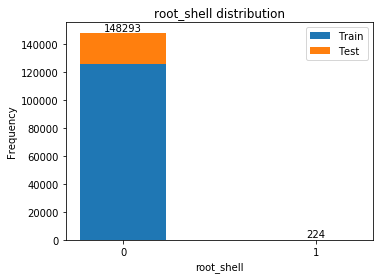
\includegraphics[width=0.9\linewidth]{img/cat3.png}

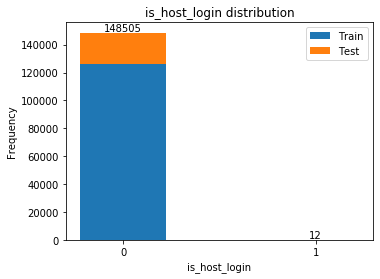
\includegraphics[width=0.9\linewidth]{img/cat4.png}

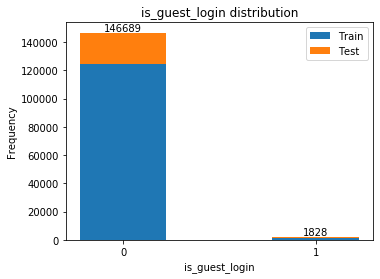
\includegraphics[width=0.9\linewidth]{img/cat5.png}

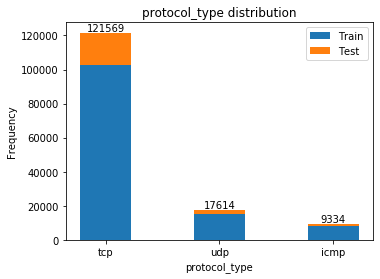
\includegraphics[width=0.9\linewidth]{img/cat7.png}
      
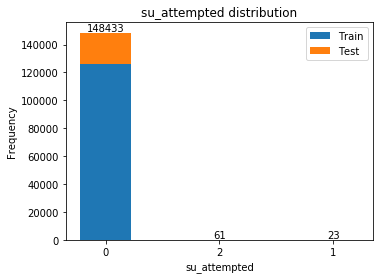
\includegraphics[width=0.9\linewidth]{img/cat8.png}

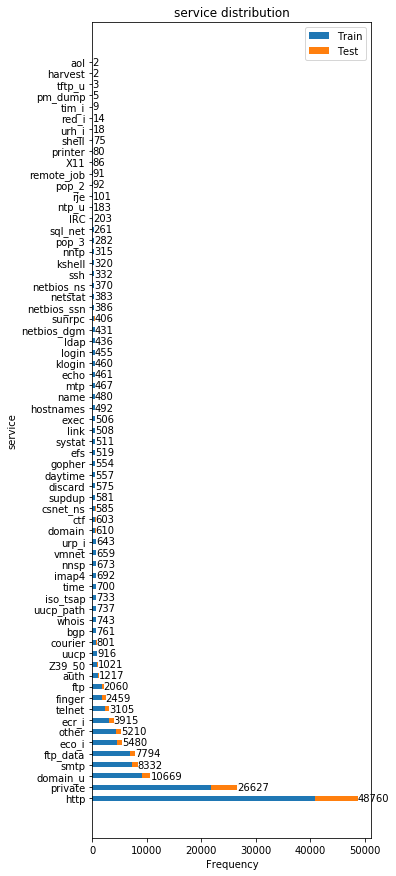
\includegraphics[width=0.9\linewidth]{img/cat10.png}

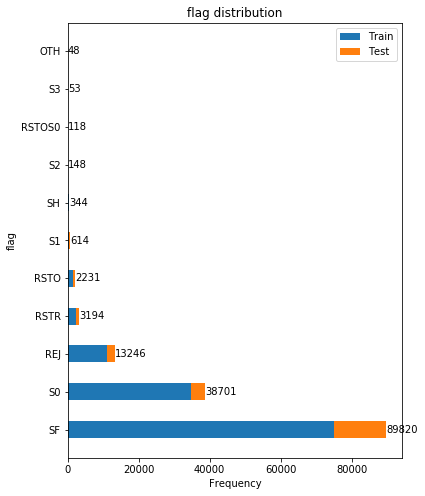
\includegraphics[width=0.9\linewidth]{img/cat9.png}

\FloatBarrier

%-------
\subsection{Numerical Data Distribution}

Numerical features have very different meanings in this dataset, and consequently different ranges. Continuous features are used for rates (e.g. error rates) and discrete features give information about the number of bytes in the packet, the connection duration, the number of reconnections and many other variables.

Figure~\ref{fig:contdist} represents the normalized dataset: each column's value has been normalized between 0 and 1 in order to visualize how the different values of each feature are distributed. Note that this normalization takes into account both the train and the test set, hence it can be used only for data analysis. Section~\ref{subsec:norm} describes how the train and test set have been normalized for learning. 

\begin{figure}[h]
    \centering
    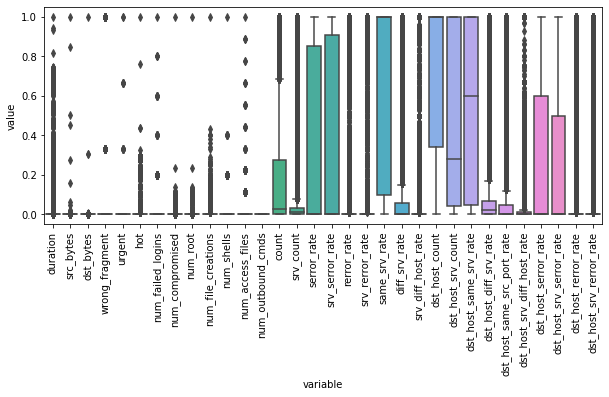
\includegraphics[width=\linewidth]{img/box-norm.png}
    \caption{Distribution of discrete and continuous values in the normalized dataset.}
    \label{fig:contdist}
\end{figure}
\FloatBarrier


%-------
\subsection{Correlation Matrix}

As a final step of the data analysis, we ran a correlation analysis for all the features of the dataset. Figure~\ref{fig:corr} illustrates the correlation matrix. Focusing on the \textit{class} column, we can see how each feature is correlated with the target variable, either directly or inversely. This analysis can be extremely useful when performing feature selection to estimate how many important features there are in the dataset.

\FloatBarrier

\begin{figure}[h]
    \centering
    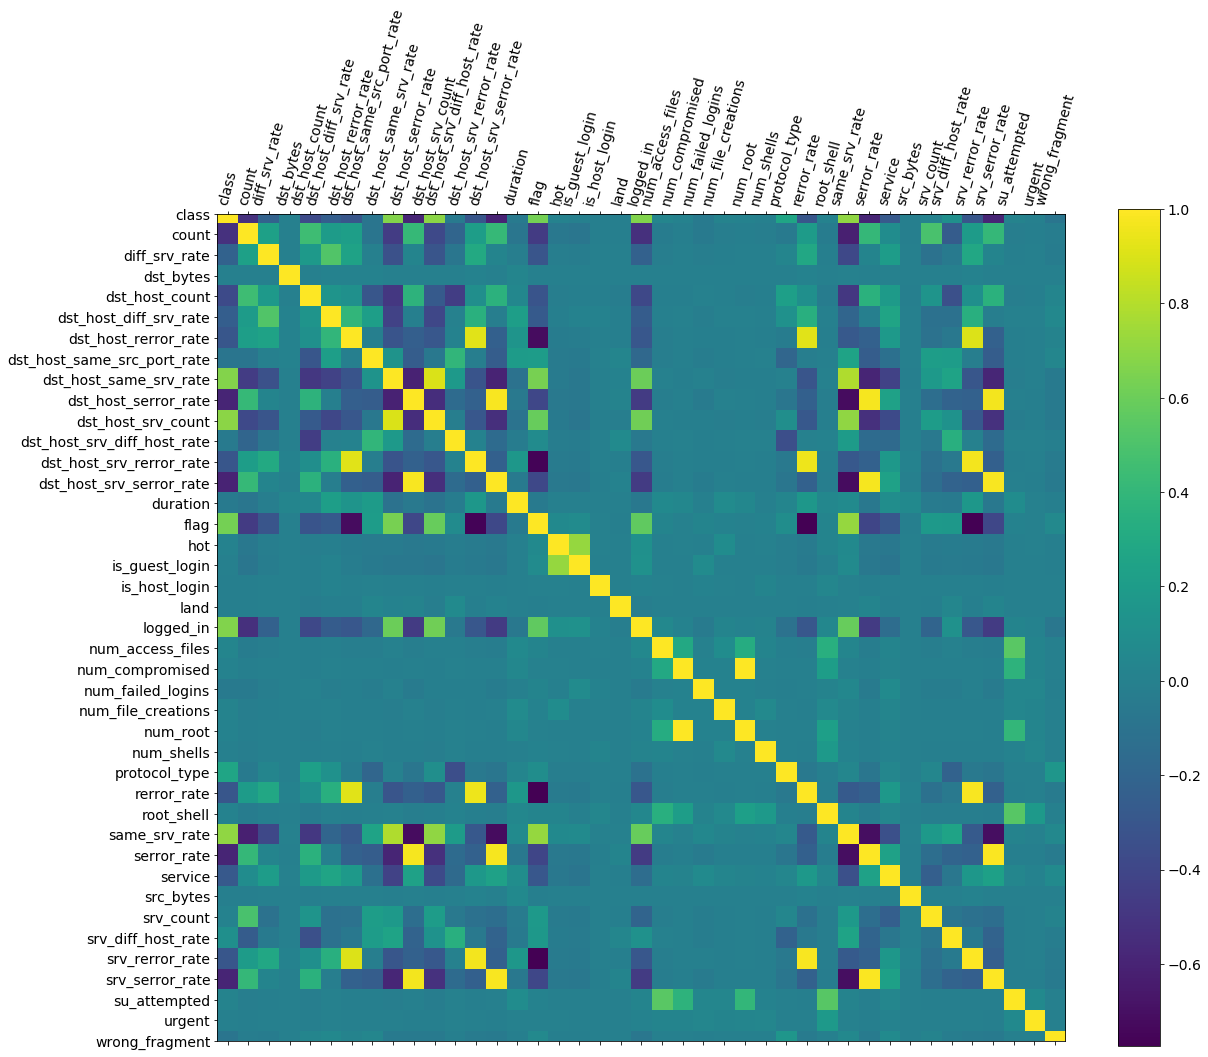
\includegraphics[width=0.9\linewidth]{img/corr1.png}
    \caption{Correlation matrix between each feature of the dataset. A brighter color means higher correlation.}
    \label{fig:corr}
\end{figure}

\FloatBarrier